\begin{Problem}
	Betrachten Sie die folgenden Familien von Kraftfeldern auf geeigneten Definitionsbereichen $D_\eta^{(n)}  \subseteq \R^3$
	\begin{align*}
		F_\eta^{(1)}:& D_\eta^{(1)}\ni \va x\to r^\eta\cdot \va x\in \R^3\\\marginnote{Eigentlich ist $\va x$ als $\va x = (x,y,z)^T$ definiert. Deswegen sind alle meine Antworten nicht die erwartete Antwort.}
		F_\eta^{(2)}:& D_\eta^{(2)}\ni\va x \to r_{12}^\eta\cdot(x_1\va e_1-x_2\va e_2)\in \R^3\\
		F_\eta^{(3)}:& D_\eta^{(3)}\ni \va x\to r_{12}^\eta\cdot\left( x_2\va e_1-x_1\va e_2 \right) \in\R^3\\
		F_\eta^{(4)}:&D_\eta^{(3)}\ni \va x\to r_{12}^\eta\cdot\left( x_2\va e_1+x_1\va e_2 \right) \in \R^3
	\end{align*}
	wobei $r_{12}=\sqrt{x_1^2+x_2^2} $ und $r=\sqrt{x_1^2+x_2^2+x_3^3} $
	Skizzieren Sie die Felder $\va F_\eta^{(n)}$ als Vektorpfeile in der von den Einheitsvektoren $\va e_1$ und $\va e_2$ aufgespannten Ebene (hier genügt es, zwischen den Fällen $\eta > -1, \eta = -1$ und $\eta < -1$ zu unterscheiden). 
	
	Bestimmen Sie, abhängig von der Potenz $\eta \in \R$,
	\begin{enumerate}
		\item den maximalen Definitionsbereich $D_\eta^{(n)}$,
		\item die maximale Bereiche $C_\eta^{(n)}\subseteq D_\eta^{(n)}$, auf denen $F_\eta^{(n)}$ konservativ ist,
		\item eine Potentialfunktion $V_\eta^{(n)}:C_{\eta}^{(n)}\to \R$ mit $F_\eta^{(n)}=-\grad{V_\eta^{(n)}}$, sofern sie existiert,
		\item das Kurvenintegral
		\[I_\eta^{(n)}(R)=\int_{\gamma_R}\dd{\va\xi}\cdot\va F_\eta^{(n)}(\va\xi)\]
		über den gegen den Uhrzeigersinn umlaufenen Kreis $\gamma_R$ mit Radius $R$ und Mittelpunkt $\va0$ in der von $\va e_1$ und $\va e_2$ aufgespannten Ebene
		\begin{center}
			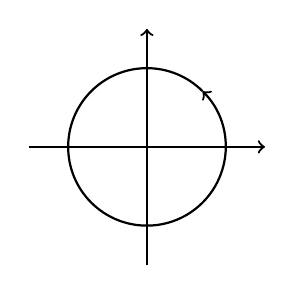
\begin{tikzpicture}
				\draw[thick, ->] (-1.5,0) -- (1.5,0);
				\draw[thick, ->] (0,-1.5) -- (0,1.5);
				\draw[thick, ->] ({1/sqrt(2)},{1/sqrt(2)}) arc (45:405:1);
			\end{tikzpicture}
		\end{center}
	\end{enumerate}
\end{Problem}


\begin{proof}
	\begin{figure}[h!]
		\begin{subcaptionbox}{$\eta>-1$}
	 {\resizebox{0.3\textwidth}{!}{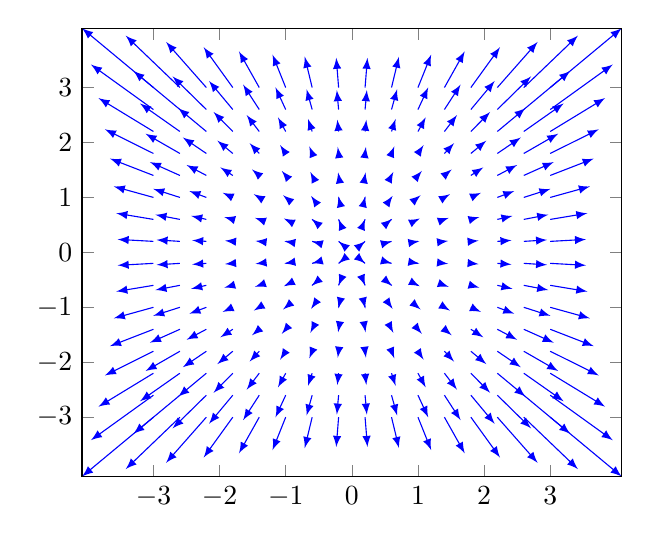
\begin{tikzpicture}
 \begin{axis}[%
  view     = {0}{90}, % for a view 'from above'
  domain   = -3:3,
  y domain = -3:3,
  xtick    = {-3,...,3},
  ytick    = {-3,...,3},
]
\addplot3[blue, quiver={u=(x*x+y*y)*x, v=(x*x+y*y)*y, scale arrows=0.02}, samples=16, -latex] (x,y,0);
\end{axis}
\end{tikzpicture}}}
	\begin{subcaptionbox}{$\eta=-1$}
	{\resizebox{0.3\textwidth}{!}{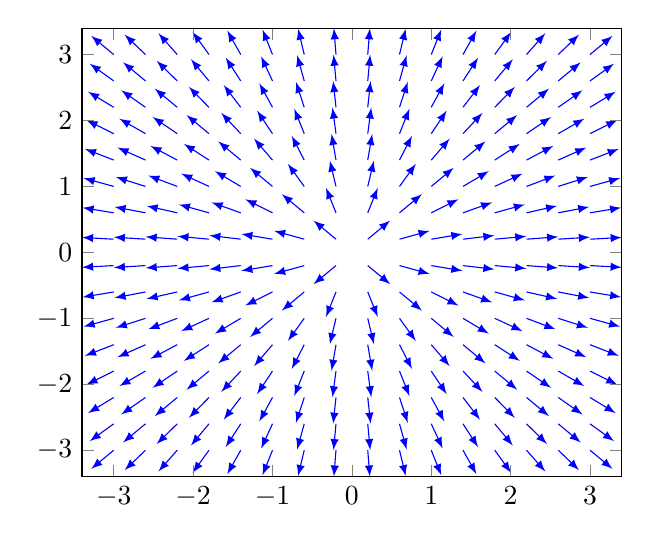
\begin{tikzpicture}
			\begin{axis}[%
				view     = {0}{90}, % for a view 'from above'
				domain   = -3:3,
				y domain = -3:3,
				xtick    = {-3,...,3},
				ytick    = {-3,...,3},
				]
				\addplot3[blue, quiver={u=x/(x*x+y*y)^(1/2), v=y/(x*x+y*y)^(1/2), scale arrows=0.4}, samples=16, -latex] (x,y,0);
			\end{axis}
	\end{tikzpicture}}}
\end{subcaptionbox}
\end{subcaptionbox}
	\begin{subcaptionbox}{$\eta<-1$}
	{\resizebox{0.3\textwidth}{!}{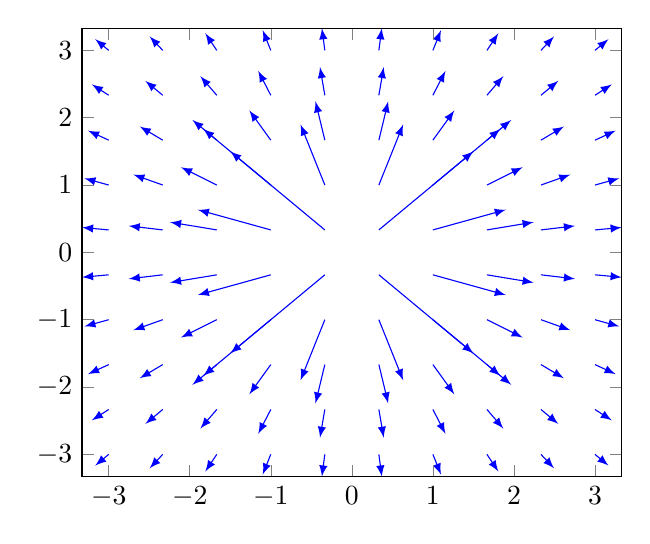
\begin{tikzpicture}
			\begin{axis}[%
				view     = {0}{90}, % for a view 'from above'
				domain   = -3:3,
				y domain = -3:3,
				xtick    = {-3,...,3},
				ytick    = {-3,...,3},
				]
				\addplot3[blue, quiver={u=x/(x*x+y*y), v=y/(x*x+y*y), scale arrows=1}, samples=10, -latex] (x,y,0);
			\end{axis}
	\end{tikzpicture}}}
\end{subcaptionbox}
\caption{Vektorpfeile f\"{u}r $\va F_\eta^{(1)}$}
\end{figure}
	\begin{figure}[h!]
	\begin{subcaptionbox}{$\eta>-1$}
		{\resizebox{0.3\textwidth}{!}{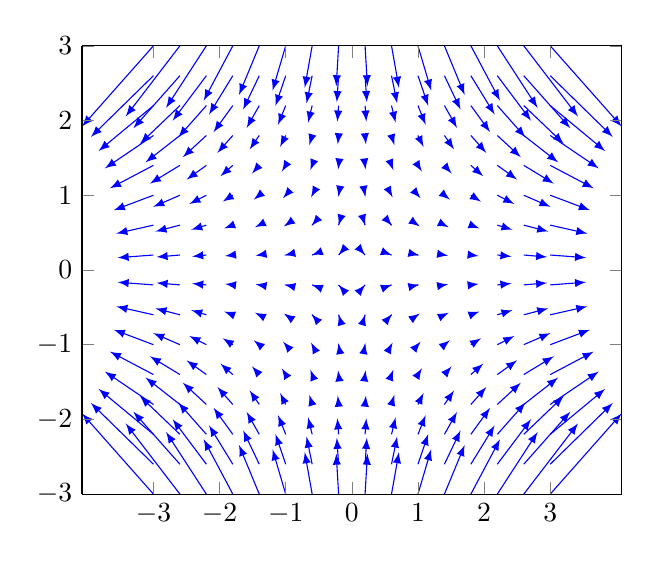
\begin{tikzpicture}
				\begin{axis}[%
					view     = {0}{90}, % for a view 'from above'
					domain   = -3:3,
					y domain = -3:3,
					xtick    = {-3,...,3},
					ytick    = {-3,...,3},
					]
					\addplot3[blue, quiver={u=(x*x+y*y)*x, v=-(x*x+y*y)*y, scale arrows=0.02}, samples=16, -latex] (x,y,0);
				\end{axis}
		\end{tikzpicture}}}
		\begin{subcaptionbox}{$\eta=-1$}
			{\resizebox{0.3\textwidth}{!}{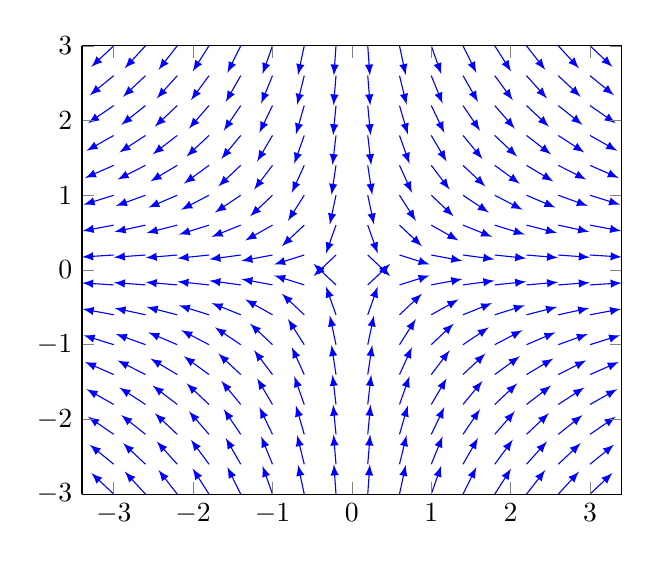
\begin{tikzpicture}
					\begin{axis}[%
						view     = {0}{90}, % for a view 'from above'
						domain   = -3:3,
						y domain = -3:3,
						xtick    = {-3,...,3},
						ytick    = {-3,...,3},
						]
						\addplot3[blue, quiver={u=x/(x*x+y*y)^(1/2), v=-y/(x*x+y*y)^(1/2), scale arrows=0.4}, samples=16, -latex] (x,y,0);
					\end{axis}
			\end{tikzpicture}}}
		\end{subcaptionbox}
	\end{subcaptionbox}
	\begin{subcaptionbox}{$\eta<-1$}
		{\resizebox{0.3\textwidth}{!}{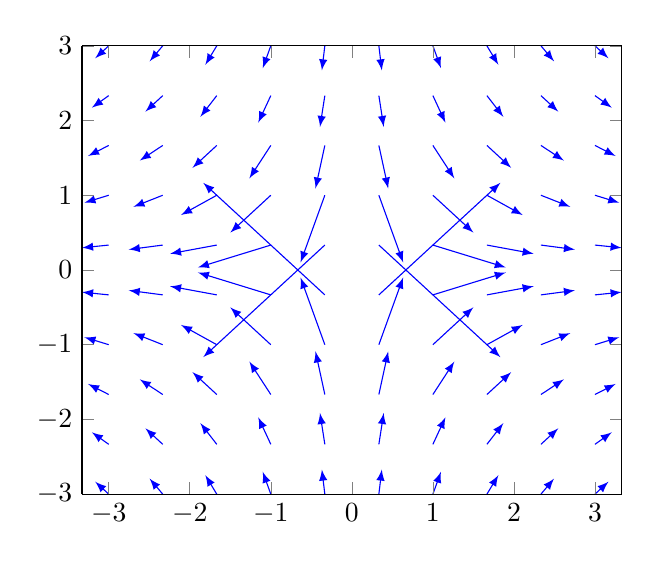
\begin{tikzpicture}
				\begin{axis}[%
					view     = {0}{90}, % for a view 'from above'
					domain   = -3:3,
					y domain = -3:3,
					xtick    = {-3,...,3},
					ytick    = {-3,...,3},
					]
					\addplot3[blue, quiver={u=x/(x*x+y*y), v=-y/(x*x+y*y), scale arrows=1}, samples=10, -latex] (x,y,0);
				\end{axis}
		\end{tikzpicture}}}
	\end{subcaptionbox}
	\caption{Vektorpfeile f\"{u}r $\va F_\eta^{(2)}$}
\end{figure}
	\begin{figure}[h!]
	\begin{subcaptionbox}{$\eta>-1$}
		{\resizebox{0.3\textwidth}{!}{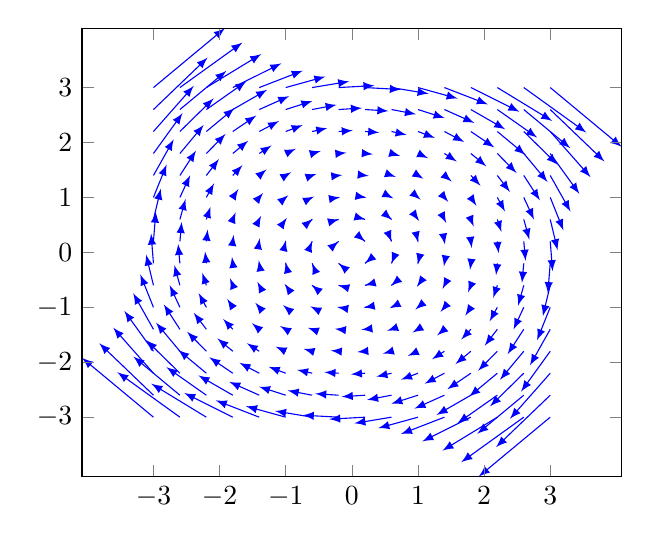
\begin{tikzpicture}
				\begin{axis}[%
					view     = {0}{90}, % for a view 'from above'
					domain   = -3:3,
					y domain = -3:3,
					xtick    = {-3,...,3},
					ytick    = {-3,...,3},
					]
					\addplot3[blue, quiver={u=(x*x+y*y)*y, v=-(x*x+y*y)*x, scale arrows=0.02}, samples=16, -latex] (x,y,0);
				\end{axis}
		\end{tikzpicture}}}
		\begin{subcaptionbox}{$\eta=-1$}
			{\resizebox{0.3\textwidth}{!}{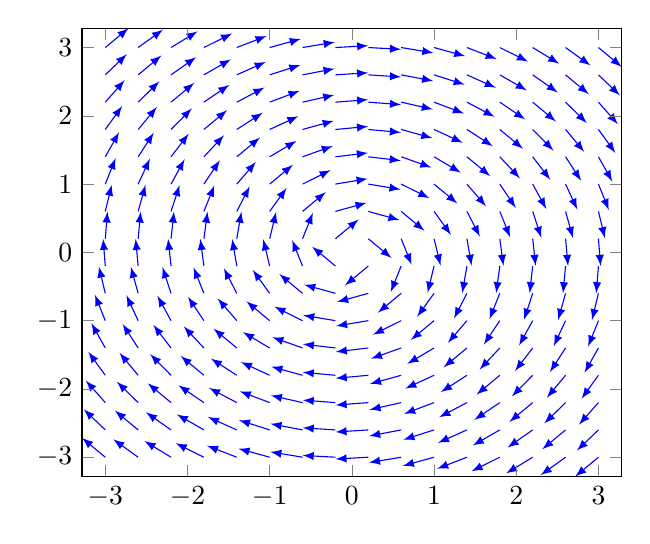
\begin{tikzpicture}
					\begin{axis}[%
						view     = {0}{90}, % for a view 'from above'
						domain   = -3:3,
						y domain = -3:3,
						xtick    = {-3,...,3},
						ytick    = {-3,...,3},
						]
						\addplot3[blue, quiver={u=y/(x*x+y*y)^(1/2), v=-x/(x*x+y*y)^(1/2), scale arrows=0.4}, samples=16, -latex] (x,y,0);
					\end{axis}
			\end{tikzpicture}}}
		\end{subcaptionbox}
	\end{subcaptionbox}
	\begin{subcaptionbox}{$\eta<-1$}
		{\resizebox{0.3\textwidth}{!}{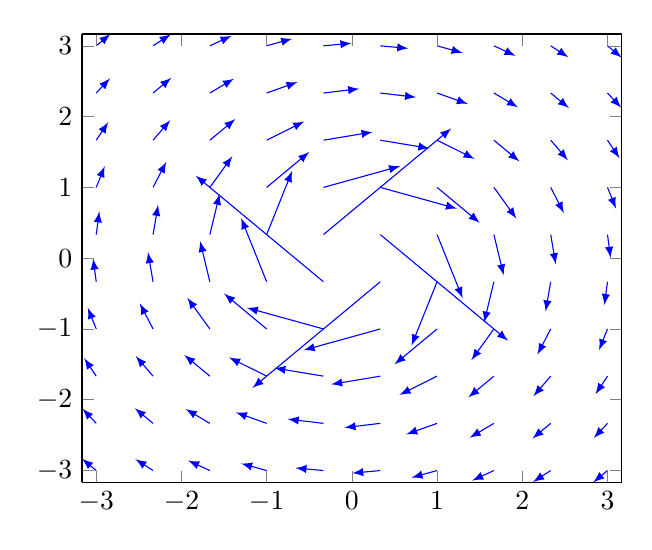
\begin{tikzpicture}
				\begin{axis}[%
					view     = {0}{90}, % for a view 'from above'
					domain   = -3:3,
					y domain = -3:3,
					xtick    = {-3,...,3},
					ytick    = {-3,...,3},
					]
					\addplot3[blue, quiver={u=y/(x*x+y*y), v=-x/(x*x+y*y), scale arrows=1}, samples=10, -latex] (x,y,0);
				\end{axis}
		\end{tikzpicture}}}
	\end{subcaptionbox}
	\caption{Vektorpfeile f\"{u}r $\va F_\eta^{(3)}$}
\end{figure}
	\begin{figure}[h!]
	\begin{subcaptionbox}{$\eta>-1$}
		{\resizebox{0.3\textwidth}{!}{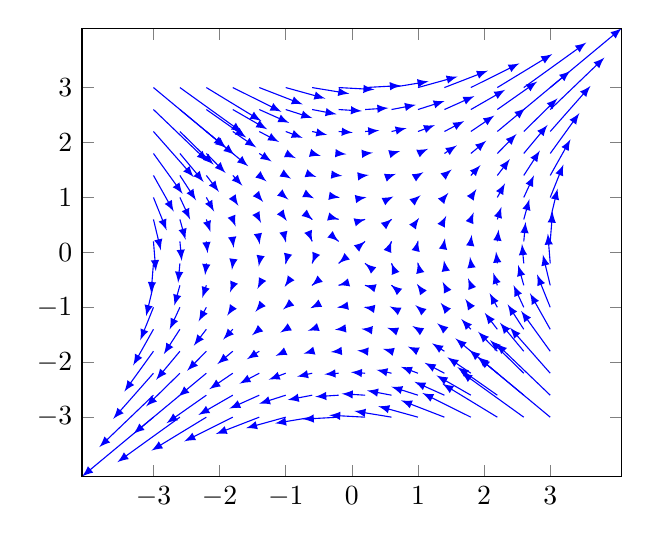
\begin{tikzpicture}
				\begin{axis}[%
					view     = {0}{90}, % for a view 'from above'
					domain   = -3:3,
					y domain = -3:3,
					xtick    = {-3,...,3},
					ytick    = {-3,...,3},
					]
					\addplot3[blue, quiver={u=(x*x+y*y)*y, v=(x*x+y*y)*x, scale arrows=0.02}, samples=16, -latex] (x,y,0);
				\end{axis}
		\end{tikzpicture}}}
		\begin{subcaptionbox}{$\eta=-1$}
			{\resizebox{0.3\textwidth}{!}{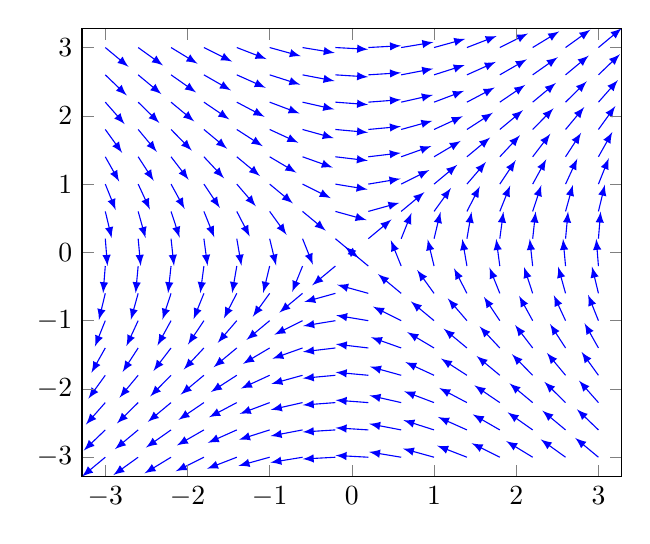
\begin{tikzpicture}
					\begin{axis}[%
						view     = {0}{90}, % for a view 'from above'
						domain   = -3:3,
						y domain = -3:3,
						xtick    = {-3,...,3},
						ytick    = {-3,...,3},
						]
						\addplot3[blue, quiver={u=y/(x*x+y*y)^(1/2), v=x/(x*x+y*y)^(1/2), scale arrows=0.4}, samples=16, -latex] (x,y,0);
					\end{axis}
			\end{tikzpicture}}}
		\end{subcaptionbox}
	\end{subcaptionbox}
	\begin{subcaptionbox}{$\eta<-1$}
		{\resizebox{0.3\textwidth}{!}{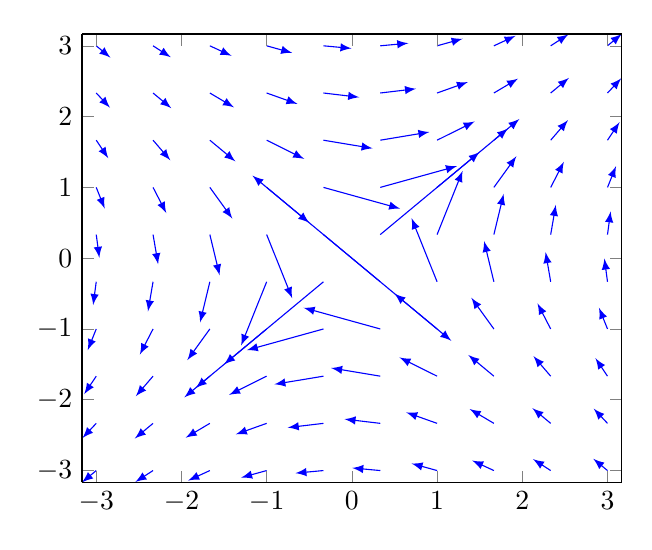
\begin{tikzpicture}
				\begin{axis}[%
					view     = {0}{90}, % for a view 'from above'
					domain   = -3:3,
					y domain = -3:3,
					xtick    = {-3,...,3},
					ytick    = {-3,...,3},
					]
					\addplot3[blue, quiver={u=y/(x*x+y*y), v=x/(x*x+y*y), scale arrows=1}, samples=10, -latex] (x,y,0);
				\end{axis}
		\end{tikzpicture}}}
	\end{subcaptionbox}
	\caption{Vektorpfeile f\"{u}r $\va F_\eta^{(4}$}
\end{figure}
\begin{enumerate}
	\item Maximalen Definitionsbereich (f\"{u}r alle $\va F_\eta^{(n)}$): Wenn $\eta\le -1, \R^3\backslash \{(0,0,0)\}$, sonst $\R^3$.
	\item maximale Bereiche, auf denen $\va F_\eta^{(n)}$ konservativ ist. $n=\dots$
	\begin{enumerate}[label=(\arabic*)]
		\item Falls $\eta=0,D_\eta^{(1)}$, sonst $z=0$\marginnote{Erwartete Antwort ist einfach $D_\eta^{(1)}$.}
		\item Falls $\eta=0, D_\eta^{(2)}$, sonst $\varnothing$
		\item Falls $\eta=-2, D_\eta^{(3)}$, sonst $\varnothing$.
		\item Falls $\eta=0, D_\eta^{(4)}$, sonst $\varnothing$.
	\end{enumerate}
	\item Potentialfunktion, f\"{u}r $n=\dots$
	\begin{enumerate}[label=(\arabic*)]
		\item Auf $z=0$ Ebene:
		
		$\eta=-2$: $V=-\frac 12\ln\left(x^2+y^2\right)$, sonst $V=-\frac 1{\eta+2}r^{\eta+2}$\marginnote{Die erwartete Antwort ist einfach $V=-\frac{1}{\eta+2}r^{\eta+2}$}

		Wenn $n=0$ kann eine Potentialfunktion f\"{u}r alle $\va r\in\R^3$ definiert werden: $V(x,y,z)=-\frac{1}{2}\left( x^2+y^2 \right) $

	\item Nur f\"{u}r $\eta=0$, $V=\frac{1}{2}\left( x^2-y^2 \right) $.
	\item F\"{u}r $\eta=-2$, $V=-\tan^{-1}\left( \frac{x}{y} \right) $.\marginnote{In zylindrische Koordinaten ist es $V=-\varphi$}

	\item F\"{u}r $\eta=0$, $V=-xy$.
	\end{enumerate}
\item Kurvenintegral, f\"{u}r $n=\dots$ 
	\begin{enumerate}[label=(\arabic*)]
		\item Weil $\curl{F_\eta^{(1)}}=0$ auf die $\va e_1, \va e_2$ Ebene, ist das Kurvenintegral stets $0$.
		\item Gleich f\"{u}r $\eta=0$. Sonst sei $x_1=\cos\theta$, $x_2=\sin\theta$, $\dd{x_1}=-\sin\theta\dd{\theta}, \dd{x_2}=\cos\theta\dd{\theta}$
			\begin{align*}
				R^\eta\int_{\gamma_R} x_1\dd{x_1}-x_2\dd{x_2}=&R^\eta \int_0^{2\pi} \left( -\cos\theta\sin\theta\dd{\theta}-\cos\theta\sin\theta\dd{\theta} \right)\\
				=& R^\eta\int_0^{2\pi}\left( -2\sin\theta\cos\theta \right) \dd{\theta}\\
				=& 0
			\end{align*}
		\item Sei $x_1=\cos\theta$, $x_2=\sin\theta$, $\dd{x_1}=-\sin\theta\dd{\theta}, \dd{x_2}=\cos\theta\dd{\theta}$
			\begin{align*}
				R^\eta\int_{\gamma_R}x_2\dd{x_1}-x_1\dd{x_2}=&R^\eta \int_0^{2\pi}\left( -\sin^2\theta\dd{\theta}-\cos^2\theta\dd{\theta} \right) \\
				=&-R^\eta \int_0^{2\pi} \dd{\theta}\\
				=&-2\pi R^\eta
			\end{align*}
			Beachten Sie, dass es f\"{u}r $\eta=-2$ ungleich $0$ ist, weil $\curl{\va F_\eta^{(3)}}$ auf $(0,0)$ nicht definiert ist.
		\item F\"{u}r $\eta=0$ ist die Kurvenintegral stets $0$. Sonst sei $x_1=\cos\theta$, $x_2=\sin\theta$, $\dd{x_1}=-\sin\theta\dd{\theta}, \dd{x_2}=\cos\theta\dd{\theta}$ und
			\begin{align*}
				R^\eta\int_{\gamma_R}x_2\dd{x_1}+x_1\dd{x_2}=& R^\eta \int_0^{2\pi} \left( -\sin^2\theta+\cos^2\theta \right)\dd{\theta} \\
				=&R^\eta \int_0^{2\pi}\cos(2\theta)\dd{\theta}\\
				=&0\qedhere
			\end{align*}
	\end{enumerate}
\end{enumerate}
\end{proof}
\begin{Problem}
	Zwischen zwei Kreisringen mit Radius $R$, die bei $x = -x_0$ und $x = x_0$ zentriert in der $yz$-Ebene liegen, sei eine Seifenhaut gespannt (s. Skizze). Aufgrund der Oberflächenspannung wird sich die Seifenhaut so ausbilden, dass die entsprechende Oberfläche minimal ist.
	\begin{enumerate}
		\item Das gesamte Problem ist rotationssymmetrisch um die $x$-Achse. Zeigen Sie, dass die Fläche der Rotationsfigur um die $x$-Achse für die Funktion $y : [-x_0, x_0] \to \R$ zwischen den Kreisringen durch
			\[
				F(y)=\int_{-x_0}^{x_0} 2\pi y(x)\sqrt{1+y'(x)^2} \dd{x}	
	\] 
	mit $y'=\dv{y}{x}$ gegeben ist.

\item Benutzen Sie nun die in der Vorlesung kennengelernte Methode der Variationsrechnung, um die Minimalfläche zu finden, die von der Seifenhaut gebildet wird. Gesucht ist also die Funktion $y$, die $F (y)$ minimiert. (Hinweis: Zeigen Sie, dass die Euler-Lagrange-Gleichung für dieses Problem als
	\[
		\frac{1}{y'}\dv{x}\left( \frac{y}{\sqrt{1+y'^2} } \right) =0\] 
		geschrieben werden kann.)
	\end{enumerate}
	\begin{center}
	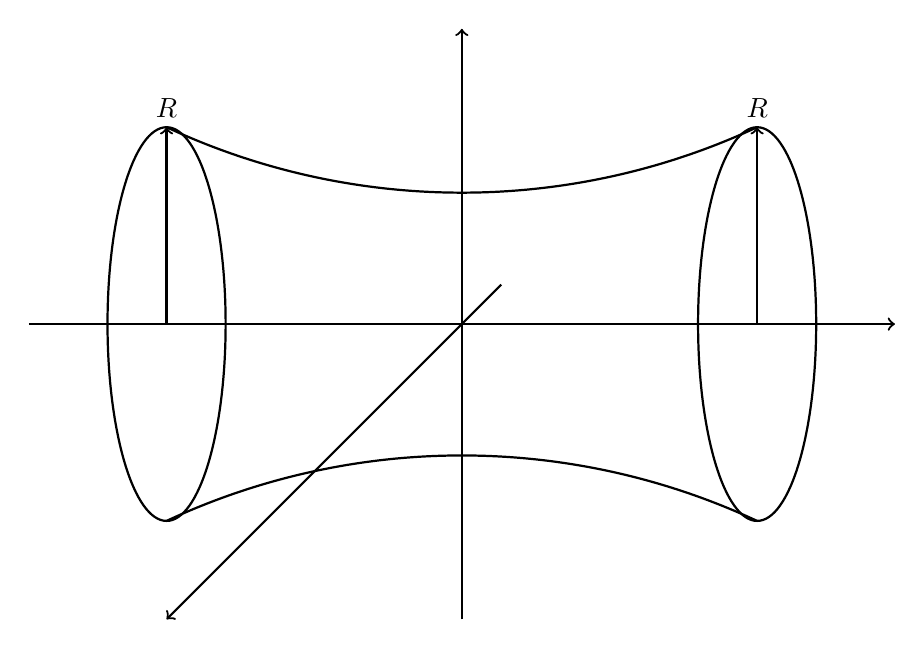
\begin{tikzpicture}[scale=2.5]
		\draw[thick, ->] (-2.2,0) -- (2.2,0);
		\draw[thick, ->] (0,-1.5) -- (0,1.5);
		\draw[thick] (-1.5,0) circle (0.3 and 1);
		\draw[thick] (1.5,0) circle (0.3 and 1);
		\draw[thick] (1.5,1) arc(-65:-115:{sqrt(3^2/(2-2*cos(50))});
		\draw[thick] (1.5,-1) arc(65:115:{sqrt(3^2/(2-2*cos(50))});
		\draw[thick, ->] (0.2,0.2) -- (-1.5,-1.5);
		\draw[thick,->] (-1.5,0) -- (-1.5,1);
		\draw (-1.5,1) node[anchor=south] {$R$};
		\draw[thick,->] (1.5,0) -- (1.5,1);
		\draw (1.5,1) node[anchor=south] {$R$};
	\end{tikzpicture}
\end{center}
\end{Problem}
\begin{proof}
	\begin{enumerate}
		\item 	\noindent \\
		
		\begin{center}
			\begin{tikzpicture}[scale=2.5]
				\draw[thick, ->] (-2.2,0) -- (2.2,0);
				\draw[thick, ->] (0,-1.5) -- (0,1.5);
				\draw[thick] (-1.5,0) circle (0.3 and 1);
				\draw[thick] (1.5,0) circle (0.3 and 1);
				\draw[thick] (1.5,1) arc(-65:-115:{sqrt(3^2/(2-2*cos(50))});
				\draw[thick] (1.5,-1) arc(65:115:{sqrt(3^2/(2-2*cos(50))});
				\draw[thick, ->] (0.2,0.2) -- (-1.5,-1.5);
				\draw[thick,->] (-1.5,0) -- (-1.5,1);
				\draw (-1.5,1) node[anchor=south] {$R$};
				\draw[thick,->] (1.5,0) -- (1.5,1);
				\draw (1.5,1) node[anchor=south] {$R$};
				\draw[thick] ({3*sin(13)/sqrt(2-2*sin(40))},0) circle (0.05 and {(-3*cos(13)+3*cos(25))/sqrt(2-2*sin(40))+1});
				\draw[thick] ({3*sin(7)/sqrt(2-2*sin(40))},0) circle (0.05 and {(-3*cos(7)+3*cos(25))/sqrt(2-2*sin(40))+1});
					\fill[pattern = north east lines] ({3*sin(7)/sqrt(2-2*sin(40))},{(-3*cos(7)+3*cos(25))/sqrt(2-2*sin(40))+1}) arc (-83:-77:{sqrt(3^2/(2-2*cos(50))}) arc (90:-90:0.05 and {(-3*cos(13)+3*cos(25))/sqrt(2-2*sin(40))+1}) arc (77:83:{sqrt(3^2/(2-2*cos(50))}) arc (-90:-270:0.05 and {(-3*cos(7)+3*cos(25))/sqrt(2-2*sin(40))+1});
					\draw[thick, <->] ({3*sin(13)/sqrt(2-2*sin(40))},{(-3*cos(13)+3*cos(25))/sqrt(2-2*sin(40))+1+0.1}) -- ({3*sin(7)/sqrt(2-2*sin(40))},{(-3*cos(13)+3*cos(25))/sqrt(2-2*sin(40))+1+0.1});
					\draw ({0.5*(3*sin(13)+3*sin(7))/sqrt(2-2*sin(40))},{(-3*cos(13)+3*cos(25))/sqrt(2-2*sin(40))+1+0.1}) node[anchor=south] {$\dd{x}$};
			\end{tikzpicture}
		\end{center}
		\[\dd{V}=2\pi y(x)\sqrt{1+y'(x)^2}\dd{x}\]
		\item 
			\begin{Theorem}
				Im Allgemein, f\"{u}r $\pdv{L}{t}=0$, gilt
				\[
					\dv{t}\left( \pdv{L}{\dot{q}}\dot{q}-L \right) =0
				.\] 
			\end{Theorem}
			\begin{proof}
				Erinnern Sie sich daran, dass
				\begin{equation}\label{eq:theorMechanik2-1}
					\dv{t}\pdv{L}{\dot{q}}=\pdv{L}{q}
				\end{equation}
				Es gilt 
				\begin{align*}
	\dv{t}\left( \pdv{L}{\dot{q}}\dot{q}-L \right) =&\left( \dv{t}\pdv{L}{\dot{q}} \right) \dot{q}+\pdv{L}{\dot{q}}\ddot{q}-\pdv{L}{\dot{q}}\ddot{q}-\pdv{L}{q}\dot{q}+\cancel{\pdv{L}{t}}\\
	=&\left( \dv{t}\pdv{L}{\dot{q}} \right) \dot{q}-\pdv{L}{q}\dot{q}\\
	=&\left( \pdv{L}{q} \right) \dot{q}-\pdv{L}{q}	\dot{q}=0\qedhere
	\end{align*}
			\end{proof}
			Sei jetzt $L(y(x),y'(x),x)=y(x)\sqrt{1+y'(x)^2} $. Es folgt $\pdv{L}{x}=0$. Daraus folgt
			\begin{align*}
				\pdv{L}{y'}y'-L=&\left( \frac{y(x)y'(x)}{\sqrt{1+y'(x)^2} } \right) y'-y(x)\sqrt{1+y'(x)^2}\\
				=&\left( \frac{yy'^2}{\sqrt{1+y'^2} } \right) -\frac{y(1+y'^2)}{\sqrt{1+y'^2} }\\
				=&\frac{-y}{\sqrt{1+y'^2} }
			\end{align*}
			Es gilt dann, dass
			\[
				\dv{x}\left( \frac{y}{\sqrt{1+y'^2} } \right) =0
			.\] 
			Daraus folgt:
			\begin{align*}
				\alpha y=&\sqrt{1+y'^2} \\
				\alpha^2 y^2=& 1+y'^2\\
				y'=&\pm \sqrt{\alpha^2y^2-1} & +\text{ wenn }x>0\\
				\int\dd{x}=&	\int \frac{\dd y}{\sqrt{\alpha^2y^2-1} }\\
				x=&\frac{1}{\alpha}\cosh^{-1}\left( \alpha y \right)-\beta\\
				y=&\frac{1}{\alpha}\cosh(\alpha(x+\beta))
			\end{align*}
			Die Randbedingungen ergeben:
				\[\alpha R=\cosh\left( \alpha(x_0+\beta) \right) =\cosh\left( \alpha(-x_0+\beta) \right) 
				\]
				Daraus folgt $\beta=0$. Leider ist die Gleichung f\"{u}r $\alpha$ unl\"{o}sbar. Die L\"{o}sung zu die Gleichung ist
				\begin{align*}
					y(x)=&\frac{1}{\alpha}\cosh(\alpha x)\\
					\alpha R=&\cosh(\alpha x)\qedhere
				\end{align*}
	\end{enumerate}
\end{proof}
